\section{Results}

\subsection{Messages size}

Hereafter we list the messages peers exchange in Multipong and their
size\footnote{the size shown in the table has to be intended as ``greater or
equal than''}:

\begin{table}[H]
  \centering
  \begin{tabular}{l|c c}
  & \textbf{\textit{Message}} & \textbf{\textit{Size [B]}}  \tabularnewline
            \hline
            \multirow{5}{*}{TCP} & \multicolumn{1}{c}{\texttt{ARE\_YOU\_HOST}} & \multicolumn{1}{c}{60} \\\cline{2-3}
                                 & \multicolumn{1}{c}{\texttt{AVAILABLE}} & \multicolumn{1}{c}{100} \\\cline{2-3}
                                 & \multicolumn{1}{c}{\texttt{CANCEL}} & \multicolumn{1}{c}{56} \\\cline{2-3}
                                 & \multicolumn{1}{c}{\texttt{DISCOVERY}} & \multicolumn{1}{c}{82} \\\cline{2-3}
                                 & \multicolumn{1}{c}{\texttt{JOIN}} & \multicolumn{1}{c}{54} \\\hline
            \multirow{3}{*}{UDP} & \multicolumn{1}{c}{\texttt{KNOWN\_HOSTS}} & \multicolumn{1}{c}{90} \\\cline{2-3}
                                 & \multicolumn{1}{c}{\texttt{STARTING}} & \multicolumn{1}{c}{187} \\\cline{2-3}
                                 & \multicolumn{1}{c}{\texttt{TELL\_IP}} & \multicolumn{1}{c}{57} \\\hline
        \end{tabular}
  \caption{Messages size}
  \label{tab:sizes}
\end{table}

\subsection{Energy and traffic}

The average power consumption and Wi-Fi direct traffic can be seen in Figure
\ref{fig:comparison}.

\begin{figure}[H]
  \centering
  \begin{tabular}{@{}c@{}c}
      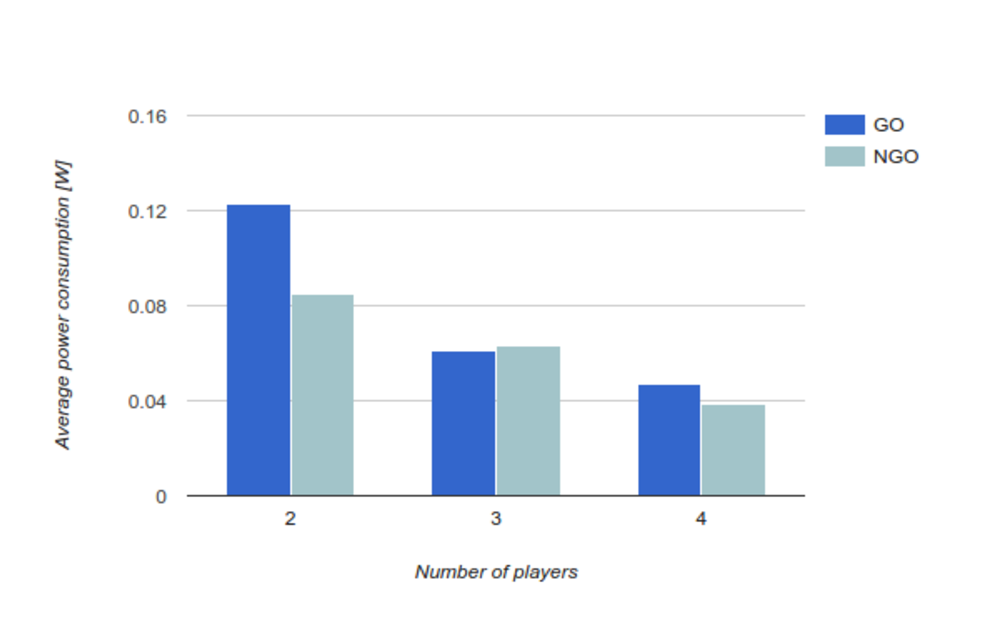
\includegraphics[width=.5\columnwidth]{img/energy.eps}
      \label{fig:energy}
    &
    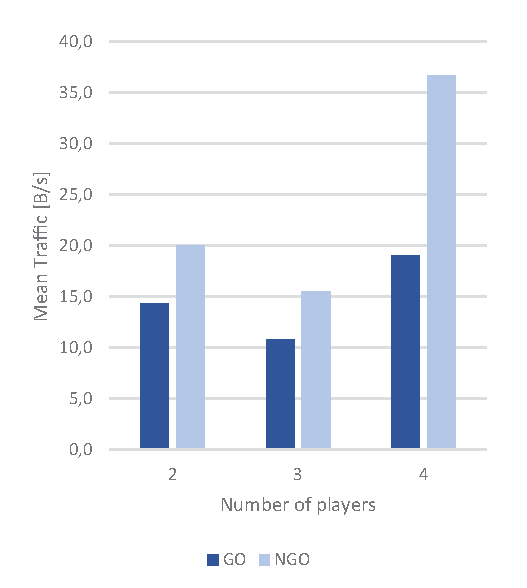
\includegraphics[width=.5\columnwidth]{img/traffic.eps}
    \label{fig:traffic}
  \end{tabular}
  \caption{GO/NGO comparison for energy and traffic}\label{fig:comparison}
\end{figure}

We notice that we have a lot of variability in power consumption because of
many factors, among which (1) the network instability, (2) user interaction
(the more the user touches the screen, the more power is consumed) and (3)
PowerTutor is not a truly reliable instrument to measure battery consumption 
because we used different devices from the ones used to create
PowerTutor's mathematical model. Hence, we can not say too much about how power
consumption varies depending on the number of players. Still, we noticed that
Multipong is quite light compared to other multimedia applications in terms of
battery consumption.

On the other hand, the figures about Wi-Fi traffic reveal that the number of
packets exchanged among the devices increases with the number of players. Often
the GO incurs less traffic than an NGO: we think this is because of iterated
attempts made by the NGOs to concurrently communicate to the GO, whereas
there is far less traffic (on average) when the GO has to send packets. In
particular, we are referring to both the liveness checks and the protocol
employed in the gameplay phase, since the GO has to spread information to all
the participants, which are diligently waiting for it.

\subsection{TCP and UDP comparison}

In Figure \ref{fig:TCP-UDP}, we can see the difference between the mean RTTs of
TCP and acked UDP transmissions.

\begin{figure}[H]
  \centering
  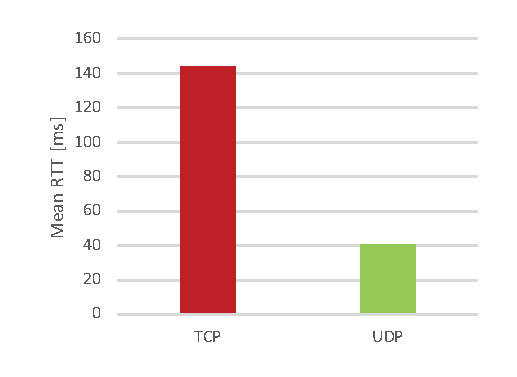
\includegraphics[width=.8\columnwidth]{img/UDPvsTCP-RTT.eps}
  \caption{TCP vs. UDP}
  \label{fig:TCP-UDP}
\end{figure}

As it can be easily seen, acked UDP is very efficient compared to TCP and
therefore we can acknowledge that acked UDP is the most suitable choice (between
these two) in the gameplay phase, whilst TCP is fit for the game formation
phase, when we do not need low latency but more reliable packet delivery.
